\section{Experiments}
\label{sec:pending-studies}
\label{sec:evidence}
The experiments follow the distinction between a predictor, an action class and a registration. We first compare fitted prediction with simpler competing explanations. On complete banks, we then compute the independent linear and orthogonal optima and bound the exact-action optimum. We also evaluate the transfer of a constructed action and compare coherent registrations. A final study compares two predictive fitting objectives on a new set of authored contexts.

\subsection{Models, coordinate banks, and evaluation design}
\label{sec:design}
We analyze six frozen base checkpoints, rather than their instruction-tuned variants: Llama-3.2-1B/3B \citep{meta2024llama32}, Llama-3.1-8B \citep{grattafiori2024llama3}, and Qwen2.5-1.5B/3B/7B \citep{qwen2025technical}. All are pretrained decoder-only autoregressive Transformers. Four normalized depth slots, $0.2,0.4,0.6,0.8$, give 24 model/readout conditions per domain. Coordinate estimation and predictor fitting are performed separately for each study, domain, model, readout and training split. In the linear-map comparisons, the fitted matrix family is shared across templates within each condition. The primary coordinate dimension is 16; the spectral sensitivity comparison uses the first eight coordinates of the same saved PCA. The state-span readout and training-only PCA follow \cref{sec:setup}. Study~1 extracts activations in FP16 and Study~2 in BF16.

The data constructions serve different purposes. The structural-recovery bank (Study~1) contains 40 short templates per domain. Each of five seeded partitions allocates 28 to training, six to diagnostic validation and six to testing, keeping all states of a template together. The coordinate bank (Study~2) uses a separate grammar construction with 48 training, 16 validation and 64 test families, each comprising two paired variants and complete state sets. Its 64 test families contribute 128 complete state blocks per condition. Those blocks support both predictor evaluation and the finite-bank spectral calculation, with different losses. A separate 64-family authored bank is used for the context-transport comparison and is held out from predictor fitting and selection.

\hypertarget{par:estimation}{}
Study~1 ridge fits no-intercept maps with coefficient $0.01$. Joint starts from these maps and uses AdamW \citep{loshchilov2019decoupled} to optimize the small matrices with soft prediction and algebraic penalties; the language model stays frozen. Generator-only fitting withholds supervision for nongenerator elements. For evaluation, Study~1 normalizes each squared prediction error by its target row's squared norm plus a fixed numerical constant (\cref{eq:D}). The compact-coordinate prediction endpoint in Study~2 normalizes by the training coordinate energy about the training mean. It averages losses over changed states within each nonidentity action, then gives the actions equal weight. The context-difference endpoints have separate aggregation rules, described in \cref{sec:new-context}. Held-out prediction keeps the training-derived coordinate transforms and fitted predictors fixed. The class-risk analysis uses the evaluated bank's own empirical second moment and a full-group average, including the identity element and fixed-point pairs.

All spectral means give equal weight to the 24 conditions in a domain and dimension; the orthogonal comparison includes all 96 units formed by two domains, two dimensions and 24 conditions. These models and readouts form a selected panel, and Study~1's five overlapping partitions are not five independent datasets. Reported bootstrap ranges describe sensitivity under the recorded resampling scheme, rather than calibrated population coverage. In the new-context comparison the unit is a paired family, retaining its measurements across models, readouts and domains together. Counts of winning conditions are descriptive panel summaries. Implementation parameters, prompts, partitions and historical resampling rules are collected in \cref{app:methods}; the Study~2 banks and follow-up designs, including paired-family resampling, are documented in \cref{app:characterization,app:pending-protocols}.

\subsection{Predictive recovery and competing explanations}
\label{sec:characterization}
\paragraph{Shared maps predict familiar transformations.}
Independent ridge predicts held-out Study~1 representations with mean $\Eeq=0.04830$ for C7 and $0.05200$ for D4. Joint yields $0.04934$ and $0.05286$: the group penalties slightly increase mean direct-prediction error on this panel. Joint lowers the mean data-space relation aggregate defined in \cref{app:metrics}. The data and operator relation diagnostics use distinct formulas and should be interpreted separately. Predictive fit and these consistency diagnostics can respond differently to the fitting objective, while their relationship also depends on operator norms and normalization denominators.

With only generator supervision, matrix products predict five excluded nonidentity elements in each group. Their errors are $0.074443/0.056558$ for C7/D4; directly fitting those same elements in that comparison gives $0.051124/0.050032$. The generator-composed prediction errors are well below those of the identity controls. Direct Ridge receives element-specific training pairs that are withheld from the generator-only fit. The comparison tests transfer to held-out action elements and templates with a fixed, already-seen state vocabulary. Detailed structural endpoints are in \cref{app:results}.

\paragraph{Category information provides a competitive explanation.}
The lexical comparison on Llama-3.2-1B and Qwen2.5-1.5B gives near-exact fits for lexical embeddings and larger errors for internal representations at matched training projected ranks of $q=6$ for C7 and $q=3$ for D4. The lexical readout reuses one vector per state across templates. The audited centered lexical spans have rank $n-1$ for $n$ states and therefore admit a linear realization of every state permutation (\cref{prop:finite,app:lexical-rank}). This supports a category-code explanation for the near-exact predictive fits. Equal projected rank does not equalize the amount or kind of retained information, and these fitted errors do not establish an exact orthogonal action.

A training-centroid control in Study~2 makes category information explicit. It decodes the source state by its nearest training centroid and shifts the source by the difference between target and source centroids. In the compact comparison, its mean losses are $0.012013/0.063821$, versus ridge's $0.014897/0.041919$. The centroid predictor wins in 9/24 C7 and 2/24 D4 conditions: its better weekday mean is not a uniform improvement. It additionally receives explicit construction state labels and an exact action table; the coordinate predictors receive supervised source--target pairs and the requested action. Its competitiveness demonstrates an available predictive explanation under this extra information. It does not establish that the frozen language model itself performs centroid decoding.

Capacity also changes the comparison. Random Fourier feature (RFF; \citealp{rahimi2007random}) and Nystr\"om \citep{williams2000nystrom} predictors fit the target-minus-source displacement using all training pairs for each fitted nonidentity action, including fixed points, then add it to the source. Neither improves both domain means at the linear storage budget with the identity map omitted from storage. Among the evaluated budgets, the first crossings below Ridge in both domain means occur at $2\times$ for Nystr\"om and $4\times$ for RFF. This budget counts predictor parameters, features, normalizers and lookup data, excluding shared PCA, model weights and runtime memory. All declared budgets are reported; these crossings describe the evaluated curves and do not define a test-selected operating point. The storage accounting does not establish equal statistical capacity or total memory use. Nor does nonlinear predictive accuracy establish a nonlinear group action. The complete budget curves and comparator definitions are in \cref{app:reproduction}.

\paragraph{A coherent alternative remains predictive.}
In Study~1, corrupting training correspondences and refitting ridge worsens prediction of the unchanged true test targets. In Study~2, conjugating the action by a fixed state-label swap defines a second consistent task and preserves group laws and fixed-point counts. Ridge losses for prescribed/alternative correspondences are $0.014897/0.017503$ for C7 and $0.041919/0.041871$ for D4. Both tasks use the same source bank and have their own targets and changed-state masks. In D4, the swap can change which corners move under a given action. The alternative's competitive prediction motivates asking how exceptional the prescribed action is among \emph{all} images in the declared comparator class. \Cref{app:predictive-controls,app:reproduction} gives the control definitions; disrupting a training correspondence and changing to a coherent target action answer different questions.

These comparisons concern fitted predictors. We next ask what error is unavoidable for any exact orthogonal action on the complete Study~2 test bank. This class comparison uses the bank's own second-moment whitening and the full-group loss in \cref{eq:class-loss-main}. Its normalization and averaging differ from the preceding predictive endpoints.

\subsection{Exact-action cost in observed representation banks}
\label{sec:observed-risk}
% Presentation only: select and round previously saved means.
\begin{table*}[t]
\caption{\textbf{Same-bank risks and constraint costs.} Each row averages all 24 fixed model/readout conditions on the Study~2 test banks. Panel (a) bounds the joint cost of exact laws and orthogonality; panel (b) separates the computed orthogonality cost $\beta$ from bounds on further common-law cost. Endpoints are computed per condition before averaging. The last column uses the fixed tolerance $\tau=10^{-8}+10^{-7}|\ell^-|$. Intervals bound mean class optima; they are not confidence intervals or measured optima. Each dimension uses its own second-moment-whitened metric.}
\label{tab:core-risk-summary}
\centering\small
\setlength{\tabcolsep}{4pt}
\textbf{(a) Joint constraint cost, $r=16$}\par\smallskip
\begin{tabular}{@{}lrrrr@{}}
\toprule
Domain & Mean $\eta$ & Mean $L^\star$ bounds & Mean $L^\star-\eta$ bounds & Mean $L(I)$ \\
\midrule
$C_7$ & 0.02563 & [0.02980, 0.05863] & [0.00416, 0.03300] & 0.76012 \\
$D_4$ & 0.10321 & [0.12944, 0.24895] & [0.02624, 0.14574] & 0.52932 \\
\bottomrule
\end{tabular}
\par\medskip
\textbf{(b) Independent orthogonality and further group-law cost}\par\smallskip
\begin{tabular}{@{}rlrrrr@{}}
\toprule
$r$ & Domain & Mean $L_{\rm orth}$ & Mean $\beta$ & Mean $L^\star-L_{\rm orth}$ bounds & $\ell^->\tau$ \\
\midrule
16 & $C_7$ & 0.028706 & 0.003074 & [0.001097, 0.029927] & 23/24 \\
16 & $D_4$ & 0.127737 & 0.024531 & [0.001842, 0.121209] & 23/24 \\
8 & $C_7$ & 0.096717 & 0.029571 & [0.035397, 0.151842] & 22/24 \\
8 & $D_4$ & 0.080819 & 0.010217 & [0.000052, 0.076930] & 19/24 \\
\bottomrule
\end{tabular}
\end{table*}


We evaluate the class-risk quantities on the original complete Study~2 test banks, without within-template centering, using each bank's own empirical second moment. The computed endpoints approximate deterministic mathematical bounds for these observed distributions. They are distinct from held-out scores of training-fitted predictors. At $r=16$, the upper bound on $L^\star$ is below the identity-family risk in each of the 48 conditions. The bounds also constrain the cost relative to unconstrained linear prediction (Table~\ref{tab:core-risk-summary}a). \Cref{fig:same-metric-risks} shows both comparisons in every primary condition. The absolute risks vary across models and readouts; additive costs must be read from the same-metric decomposition, rather than from distances on the logarithmic axis.

\paragraph{Orthogonality and further common-law cost.}
\label{par:orthogonal-results}
The independent orthogonal comparison separates the computed cost $\beta$ from bounds on the further cost $L^\star-L_{\rm orth}$ (Table~\ref{tab:core-risk-summary}b). At $r=16$, the latter's lower endpoint exceeds the fixed numerical tolerance in 23/24 conditions per domain. The computed lower bounds indicate an additional group-law cost in those conditions under the stated assumptions and numerical checks. The tolerance classifies the computed endpoints; it is not a rigorous bound on propagated numerical error. The interval bounds the remaining cost without determining its exact value.

At $r=8$, the corresponding counts are 22/24 for C7 and 19/24 for D4; one C7 endpoint is only $1.55$ times its tolerance. All nine zero lower endpoints across both dimensions remain included. A zero lower endpoint is inconclusive about strict positivity. Each dimension has its own coordinates, whitening and normalization, so the comparison characterizes dependence on the retained space rather than selecting a superior dimension. Per-condition results and numerical rules are in \cref{app:orthogonal-results}.

\paragraph{The computed cost bounds are heterogeneous.}
At $r=16$, C7's joint-cost lower endpoints $p^-$ have median $0.000389$ and range $[0.0000349,0.06254]$. Two conditions---Llama-3.1-8B/layer 13 and Llama-3.2-3B/layer 11---contribute $90.7\%$ of their sum. D4's corresponding median is $0.01876$, with range $[0.00254,0.08719]$. All conditions retain equal weight. Moreover, positivity of $p^-$ follows from $\eta>0$ under the theorem; the data inform its magnitude and distribution, not a separate positivity discovery.

The further-law lower endpoints $\ell^-$ are even more uneven in C7: their median is $5.35\times10^{-6}$ and range $[0,0.026188]$, with Llama-3.1-8B/layer 13 supplying $99.44\%$ of the sum. This one-condition concentration concerns the further-law bound, whereas the two-condition $90.7\%$ concentration concerns the joint bound. Neither is a proportion of the unknown true costs. D4's further-law endpoints have median $0.000339$ and range $[0,0.012617]$. The upper bounds remain much wider, so small lower endpoints do not establish small actual costs.

\paragraph{Sensitivity to individual context families.}
For the prescribed C7 action, we delete each of the 64 complete families in every $r=16$ condition, removing both variants and their complete seven-state blocks together. All 1,536 deletions are evaluable, and the same 23/24 conditions exceed the threshold after every deletion under the original tolerance rule. Llama-3.1-8B/layer 13 retains $\ell^-\in[0.02435,0.02696]$, compared with $0.02619$ on the complete bank, and accounts for $99.38\%$--$99.48\%$ of the lower-endpoint sum. Thus both the positive-bound count and the cross-condition concentration persist across these deletions. PCA remains fixed, but each reduced bank uses its own second-moment whitening: this is sensitivity to the changed empirical distribution and metric, not additive family attribution under a fixed loss. This check does not rerank alternative images and therefore does not establish deletion stability of the registration rankings. It also does not address joint deletions or shared construction biases (\cref{app:c7-family-influence}).

% Keep the figure after the complete family-sensitivity paragraph.
\begin{figure}[H]
\centering
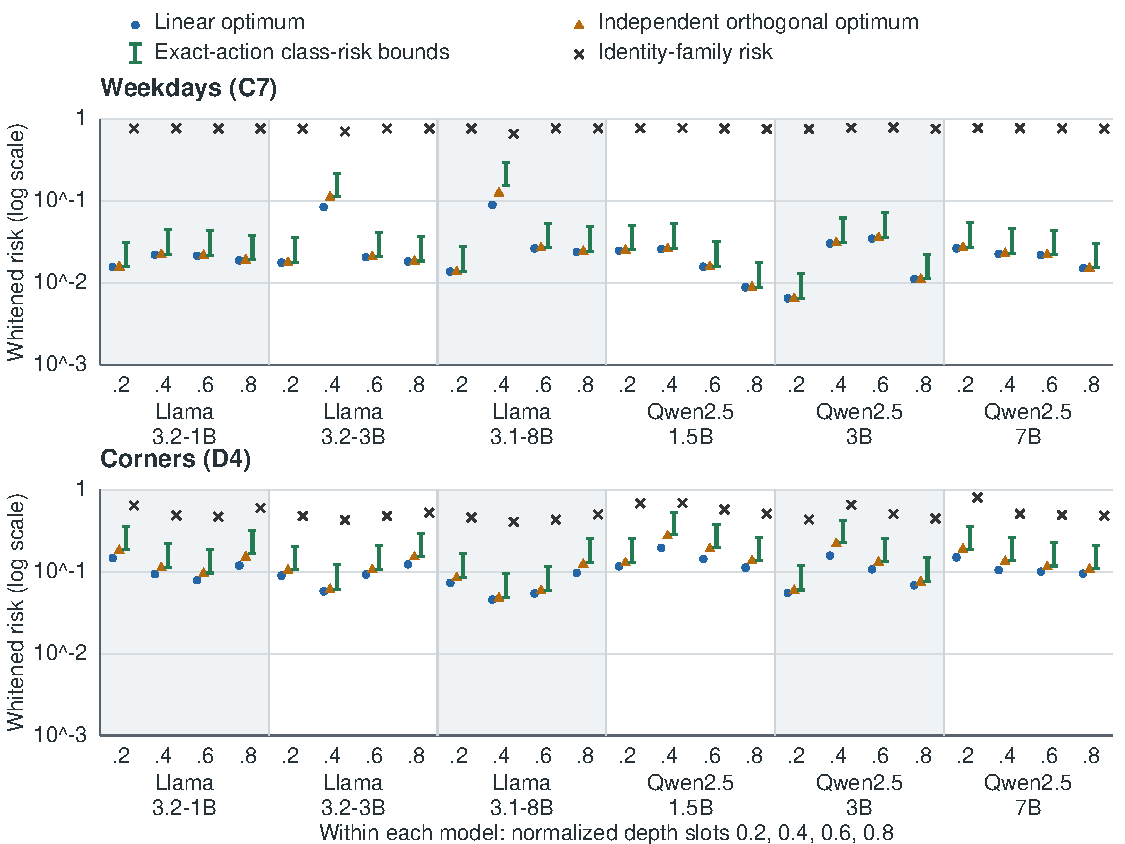
\includegraphics[width=\textwidth]{figures/same_metric_risks_v061.pdf}
\caption{\textbf{Same-metric risks in every primary condition.} Circles show $\eta$, triangles $L_{\rm orth}$, green segments $[2(1-\gamma_r),2(1-\gamma_r^2)]$, and crosses $L(I)$ at $r=16$. Within each of the 48 conditions, all four quantities use the same complete Study~2 test bank, its own second-moment whitening, and uniform state/group weights. Each model has four readouts; horizontal offsets separate symbols. The logarithmic axis shows absolute risk levels, not additive constraint costs. Segments bound the exact-action class optimum; they are neither confidence intervals nor measured witness losses. All conditions are retained. Training-metric witness transfer is reported separately in \cref{sec:witness-transfer}.}
\label{fig:same-metric-risks}
\end{figure}

\Needspace{11\baselineskip}
\paragraph{Invariant components contribute to high budgets.}
The selected trivial contributions average $b_{\rm triv}=0.61540/0.72742$ for C7/D4: much of the captured energy is invariant to the state action. These are fractions of total whitened energy, not fractions of $\gamma_r$, and need not equal the total trivial energy used by $L(I)$. Invariant components may include contextual or constant structure; state-dependent components can still encode categories. The type correction is also small in most primary conditions: the unnormalized $|\Delta_{\rm type}|$ is at most $5.33\times10^{-15}$ in 47/48. Only Llama-3.1-8B/C7/layer 13 has a material correction, with $\Delta_{\rm type}/16=0.00827$. Thus the correction to ordinary spectral truncation is concentrated at dimension 16. This correction compares the typed budget with ordinary top-$r$ truncation and does not measure the further group-law cost. A near-zero $\Delta_{\rm type}$ can coexist with a positive lower bound on $L^\star-L_{\rm orth}$. The detailed type decomposition is in \cref{app:bounded-risk-details}.

\subsection{Transfer of constructed exact actions}
\label{sec:witness-transfer}
\begin{table}[t]
\caption{Transfer of frozen predictors at $r=16$ in the training metric. These means use training whitening for both construction and old test banks, including identity and fixed points. OLS and ridge need not obey group laws. The witness is feasible, not claimed optimal. Its transfer loss is not checked against Table~\ref{tab:core-risk-summary}'s test-metric exact-orthogonal bounds: changing whitening can also change admissibility of the same raw-coordinate function.}
\label{tab:followup-witness}
\centering\small
\begin{tabular}{@{}lrrrrr@{}}
\toprule
& Construction bank & \multicolumn{3}{c}{Old test bank, frozen training metric} & Witness worse \\
Domain & Witness & Witness & OLS & Ridge & than OLS \\
\midrule
$C_7$ & 0.02906 & 0.02806 & 0.02141 & 0.02141 & 24/24 \\
$D_4$ & 0.11996 & 0.11117 & 0.08878 & 0.08878 & 24/24 \\
\bottomrule
\end{tabular}
\end{table}

The bounds concern the best member of an entire class on one bank. To evaluate an exact action as a predictor, we construct a \emph{witness}: one feasible operator family, rather than a claimed minimizer. The training bank first supplies the second-moment whitening and the type-constrained subspace selection. The construction retains complete real irreducible blocks, forms an equivariant basis, and uses orthogonal Procrustes alignment to express the resulting action in the training-whitened coordinates. For C7 this preserves complete rotation planes; for D4 it also preserves the reflection pairing of its two-dimensional type. The operators and whitening transform are then frozen for held-out evaluation.

All 48 constructions pass the specified action-law and orthogonality checks, and their construction-bank risks lie within the analytic bounds. These numerical checks verify the implemented construction at the declared tolerances; they are not interval-arithmetic certificates or evidence of class optimality.

On the held-out bank, witness losses average $0.02806/0.11117$ for C7/D4, compared with $0.02141/0.08878$ for training-fitted OLS. The witness has higher loss than OLS and fixed-coefficient ridge in every condition (Table~\ref{tab:followup-witness}). Training whitening makes the ridge baseline nearly a rescaling of the OLS matrices by $1/1.001$. Exact algebraic structure is therefore feasible here without improving this constructor's transfer performance. The ordering is empirical: class inclusion on one distribution does not force an ordering between training-fitted predictors on another.

The comparison also uses a different metric from the preceding bank bounds. Both construction and held-out witness losses retain the \emph{training} whitening, whereas Table~\ref{tab:core-risk-summary} characterizes the test bank in its \emph{own} whitening. Re-expressing the training action in test-whitened coordinates preserves its group law by conjugacy, but need not preserve orthogonality. The reported transfer losses therefore use a different metric from those intervals. Using a witness loss as a feasible-action upper bound requires evaluation under the same loss and verification that the action belongs to the corresponding exact orthogonal class. The constructor and coordinate-change derivation are given together in \cref{app:metric-conjugation}.

\subsection{Semantic registration and dimensional sensitivity}
\label{sec:registration-sensitivity}
The existence of a compatible action leaves open which candidate state-action image receives stronger spectral support. We enumerate all 120 distinct cyclic order-seven permutation-image subgroups on the weekdays and all three dihedral order-eight images on the corners, including the prescribed image. These counts concern image subgroups, not choices of generators or arbitrary inconsistent relabelings. Every candidate defines coherent transformed targets on the same source bank. Within the prescribed C7 image, the one-day, two-day and reverse generators are reparameterizations with the same full-group spectral score. The comparison therefore does not distinguish these assignments of a named generator.

On the original $r=16$ banks, the prescribed image leads all alternatives in $\gamma_r$ by more than the recorded pairwise tolerance in 7/24 C7 and 16/24 D4 conditions. To interpret these ranks, we also compare absolute score margins. For the prescribed image $H_0$, let
\[
 d_{\rm top}=\gamma_r(H_0)-\max_{H\ne H_0}\gamma_r(H),\qquad
 d_{\rm median}=\gamma_r(H_0)-\operatorname{median}_{H\ne H_0}\gamma_r(H).
\]
The median strongest-alternative margin is $-5.52\times10^{-6}$ in C7 and $5.96\times10^{-6}$ in D4 (Table~\ref{tab:bounded-margins}). C7's score spread across all images has median $3.88\times10^{-5}$ and maximum $4.07\times10^{-4}$, although the prescribed image's rank ranges from first to a numerical tie interval of 102--105 among 120. D4 spans all three ranks, with median spread $1.36\times10^{-4}$ and maximum $0.03984$. Rank changes can therefore accompany small absolute changes, particularly for weekdays. These are spectral-budget comparisons between registered tasks, not exact-$L^\star$ rankings, permutation $p$-values or semantic probabilities.

\begin{table}[t]
\caption{Registration margins in the normalized score $\gamma_r$ at $r=16$ in all 24 fixed conditions per domain. Positive margins indicate a larger score for the prescribed image than for the strongest or median alternative. U/T/B counts unique leading, tied leading and behind under the recorded pairwise tolerance. The margins compare coherent target actions.}
\label{tab:bounded-margins}
\centering\small
% Generated by analysis/main30_bounded_v1/derive.py; never edit numbers.
\begin{tabular}{llrrrc}
\toprule
Domain & Margin & Median & Min. & Max. & U/T/B \\
\midrule
C7 & $d_{\rm top}$ & $-5.52\!\times\!10^{-6}$ & $-3.03\!\times\!10^{-4}$ & $1.97\!\times\!10^{-5}$ & 7/0/17 \\
 & $d_{\rm median}$ & $1.60\!\times\!10^{-6}$ & $-4.13\!\times\!10^{-5}$ & $4.42\!\times\!10^{-5}$ &  \\
D4 & $d_{\rm top}$ & $5.96\!\times\!10^{-6}$ & $-1.23\!\times\!10^{-2}$ & $3.82\!\times\!10^{-2}$ & 16/0/8 \\
 & $d_{\rm median}$ & $1.46\!\times\!10^{-5}$ & $-2.04\!\times\!10^{-3}$ & $3.90\!\times\!10^{-2}$ &  \\
\bottomrule
\end{tabular}

\end{table}

A shared invariant component does not by itself settle this comparison. All enumerated images are transitive, so their full trivial energy $e_{\rm triv}$ is the same within a fixed bank: the invariant projection is the within-template state mean. Their selected contributions $b_{\rm triv}$ can differ because types compete for the dimension budget (\cref{sp:transitive-trivial-energy}).

A uniquely leading image still leaves its generator reparameterizations unresolved. The mechanism constructions illustrate a separate limit of exact-action compatibility. Both a shared-action construction and a stable-code construction have machine-scale noiseless witness loss, while the sampled contextual-orientation construction has smaller budgets. The stable-code construction itself supports a valid shared action. It establishes that stable coding is compatible with these diagnostics, without identifying the empirical representations with that construction or calibrating a semantic classifier (\cref{tab:followup-simulations}).

\paragraph{Sensitivity to the state-invariant component.}
We assess this dependence by subtracting the mean across states
within each complete test template in the saved 16-dimensional
Study~2 coordinates.
We compare the original observations with two centered versions,
one retaining the original test-bank whitening and the other
using the centered bank's own second-moment whitening.
For all three treatments, we rank candidate images by
$s_{16}=C_{16}/16$ and compute the strongest-alternative margin
using this score.
Table~\ref{tab:template-centering-main} reports the results.
With the original whitening retained, centering increases the
number of conditions in which the prescribed weekday image
is uniquely leading by $s_{16}$, while the prescribed corner
image falls behind an alternative in every condition.
Thus the loss of the original D4 lead already occurs under the
original whitening metric.
Rewhitening further changes the weekday leading count and the
margins in both domains.
These comparisons show that spectral preference within the
retained space depends on the inclusion of state-invariant
components and on the whitening metric.
The disappearance of a prescribed-image lead is a ranking
result and does not establish that exact actions cease to exist.
The fixed-whitening centered treatment is reported through
spectral budgets and ranks, without applying the
unit-second-moment risk bounds to its score.
The construction and numerical checks are given in
\cref{app:template-centering-sensitivity}.

\begin{table}[!htbp]
\centering
\small
\setlength{\tabcolsep}{5pt}
\caption{
Registration sensitivity to within-template centering at $r=16$.
Each domain contains 24 model--layer conditions.
The mean score refers to the prescribed image.
U/T/B counts conditions in which it is uniquely leading,
tied for the lead, or behind.
The margin is its score minus the largest alternative score,
with the median taken across conditions.
For the original and rewhitened centered treatments,
$s_{16}=\gamma_{16}$.
For centered observations retaining the original whitening,
$s_{16}$ uses the original total energy as its denominator,
rather than the remaining centered energy.
Rewhitening changes the metric.
}
\label{tab:template-centering-main}
\begin{tabular}{llrcr}
\toprule
Domain & Treatment & Mean $s_{16}$ & U/T/B
       & Median $d_{\rm top}$ \\
\midrule
$C_7$ & Original
      & 0.985102 & 7/0/17
      & $-5.52\times10^{-6}$ \\
      & Centered, original whitening
      & 0.376059 & 15/0/9
      & $+8.47\times10^{-5}$ \\
      & Centered, own whitening
      & 0.638632 & 18/0/6
      & $+8.46\times10^{-3}$ \\
\midrule
$D_4$ & Original
      & 0.935278 & 16/0/8
      & $+5.96\times10^{-6}$ \\
      & Centered, original whitening
      & 0.252296 & 0/0/24
      & $-6.76\times10^{-4}$ \\
      & Centered, own whitening
      & 0.596606 & 0/0/24
      & $-2.56\times10^{-2}$ \\
\bottomrule
\end{tabular}
\end{table}

% Format-only selection from the completed sensitivity coverage.
\begin{table}[t]
\caption{Retained-dimension sensitivity on the same complete Study~2 banks. Each row summarizes all 24 fixed conditions; $p^-$ is the lower endpoint for joint exact-law and orthogonality cost. The last column counts a uniquely highest budget for the specified semantic image among all 120 C7 or three D4 images, using the original tolerance. Eight coordinates are the leading eight saved PCA coordinates. The dimensions have different whitened metrics and normalizations; these are not optimal-dimension comparisons or significance tests.}
\label{tab:sensitivity-main}
\centering\small
\setlength{\tabcolsep}{5pt}
\begin{tabular}{@{}lrrrr@{}}
\toprule
Domain & $r$ & Mean $\gamma_r$ & Median $p^-$ & Unique leading image \\
\midrule
$C_7$ & 16 & 0.985102 & 0.000389 & 7/24 \\
$C_7$ & 8 & 0.933943 & 0.041288 & 4/24 \\
\addlinespace
$D_4$ & 16 & 0.935278 & 0.018756 & 16/24 \\
$D_4$ & 8 & 0.959581 & 0.005865 & 19/24 \\
\bottomrule
\end{tabular}
\end{table}

Retaining eight rather than sixteen coordinates changes the answer quantitatively (Table~\ref{tab:sensitivity-main}). The prescribed image is uniquely leading in 4/24 C7 and 19/24 D4 conditions, and the C7 type correction exceeds the original comparison tolerance in eight conditions rather than one. No D4 condition exceeds it at either dimension. This count applies the recorded comparison tolerance to the unnormalized $\Delta_{\rm type}$, as specified in \cref{app:spectral-dimension-sensitivity}. The absence of a consistently leading prescribed image persists, but the margins, costs and preferred images depend on the observation space. Each dimension has its own second-moment metric and $1/r$ normalization, so this is not a common-loss contest to choose an optimal dimension. The full comparison is provided in \cref{app:spectral-dimension-sensitivity}; its role is to reveal dependence on the observation space, not to tune that space for favorable results.

\subsection{Context transport under a new language construction}
\label{sec:new-context}
\begin{table}[t]
\caption{New authored contexts under matched validation selection. Losses use old-training difference energy. Negative contrasts favor difference fitting. The last column reports the 2.5th/97.5th percentiles from 2,000 paired-family bootstrap draws; it describes conditional sensitivity over 64 authored families, not calibrated population coverage. Model/readout cells and both domains remain paired in each family.}
\label{tab:followup-context}
\centering\small\setlength{\tabcolsep}{3pt}
\begin{tabular}{@{}lrrrrr@{}}
\toprule
& \multicolumn{3}{c}{Mean context-difference loss} & Difference minus & Family sensitivity \\
Panel & Identity & Coordinate fit & Difference fit & coordinate & range \\
\midrule
$C_7$ & 0.04357 & 0.05031 & 0.04448 & -0.00583 & [-0.00668, -0.00501] \\
$D_4$ & 0.16615 & 0.12273 & 0.12892 & +0.00619 & [+0.00397, +0.00841] \\
Equal-domain mean & 0.10486 & 0.08652 & 0.08670 & +0.00018 & [-0.00103, +0.00136] \\
\bottomrule
\end{tabular}
\end{table}

A separate prediction question is whether an objective that helps within one context construction also helps on new wording. For paired variants $v=0,1$ of a context family $f$, define $u_{i,f}=z_{i,f,0}-z_{i,f,1}$ and its transformed target $u_{g(i),f}$. Coordinate fitting learns a no-intercept map from $(z_{i,t},z_{g(i),t})$ and applies it to $u$. Difference fitting learns directly from $(u_{i,f},u_{g(i),f})$. Both predictors are evaluated using squared difference error divided by the same original training difference energy $E_u$. The new comparison averages changed-state losses within each nonidentity action before giving actions equal weight. Subtracting same-state representations cancels state-only components but retains context main effects, so the target is not a pure state--context interaction.

The new bank contains 64 assistant-authored paired frames per domain, or 896 weekday and 512 corner prompts per model. Both predictors are fitted on the original training families. In the new primary comparison, each predictor selects a ridge coefficient per nonidentity action using the same context-difference loss on the original validation families. Fitting and selection precede evaluation on the new bank. The earlier coordinate comparator selected a single coefficient per condition using mean coordinate validation loss across actions. The new secondary comparison changes only the coordinate arm's validation criterion to coordinate loss; the difference arm is unchanged. The coordinate arm still selects a coefficient per action, so this secondary comparison does not restore the earlier shared-coefficient rule. Its difference-minus-coordinate contrast remains negative for C7 and positive for D4. The earlier test endpoint pooled changed-state pairs, which gives D4 actions different weights from the new equal-action endpoint because actions move different numbers of corners. Thus the original and new protocols differ in wording, validation selection and, for D4, action weighting. This study evaluates predictive transport on the new contexts. The protocols are detailed in \cref{app:reproduction,app:pending-protocols}.

Difference fitting minus coordinate fitting is $-0.005833$ for C7 and $+0.006190$ for D4 on average. Difference fitting has lower loss in 20/24 weekday conditions and 8/24 corner conditions. In C7, difference fitting lowers the mean from $0.05031$ to $0.04448$, while identity has a lower mean of $0.04357$. In D4, both fitted predictors improve on identity on domain means, with coordinate fitting giving the lowest mean (Table~\ref{tab:followup-context}). With the chosen domain weights and domain-specific normalizations, the two contrasts yield an equal-domain mean of $+0.000178$, with family-resampling percentiles $[-0.001035,+0.001362]$. This resampling holds the fitted predictors and selected coefficients fixed. The domain-specific comparisons show lower loss from difference fitting for weekdays and higher loss for corners on this authored bank.

\begin{figure}[!ht]
\centering
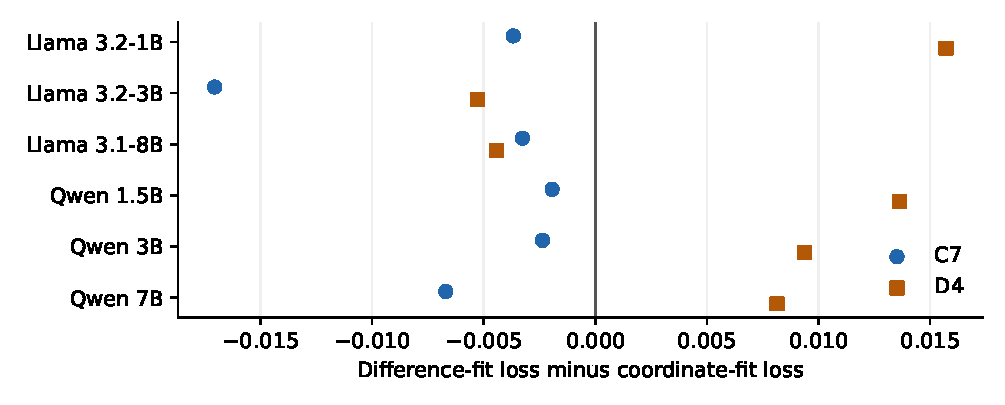
\includegraphics[width=.88\textwidth]{figures/context_transfer_followup.pdf}
\caption{New-context difference-fit minus coordinate-fit loss by model, averaged over four fixed readouts. Negative values favor difference fitting. All six weekday model means are negative, whereas four corner model means are positive. The points summarize the selected panel, not independent population draws; Table~\ref{tab:followup-context} gives the paired-family sensitivity ranges.}
\label{fig:context-followup}
\end{figure}

The frames retain the seen state vocabulary while changing outer narratives and limited factual wording. They are authored pairs, not independent human-prose samples. In a causal decoder, the state-span readout depends only on the tokenized prefix through the last selected token, as specified in \cref{sec:setup}. For D4, the difference-minus-coordinate contrast changes from $-0.015918$ under the original protocol to $+0.006190$ under the new one. The change in sign compares two protocols that vary wording, validation selection and action weighting together; it does not isolate the effect of new wording. The paired-family resampling contract is in \cref{app:pending-protocols}.

\FloatBarrier
